
\title{Wireless Sensor Network Simulation Using Tossim}  
\author{ by\\         
Alireza Mortezaei\\  
        4B Software Engineering, University of Waterloo \\ 
        Supervised by\\ 
        Dr. Mahesh Tripunitara 
}  
\date{\today}  
  
\documentclass[11pt, titlepage, oneside]{article}  
\linespread{1.5} 
\usepackage{graphicx}  
\usepackage{amssymb}  
\usepackage{amsmath}  
\usepackage{color} 
\usepackage{xcolor} 
\usepackage{listings} 
\usepackage{caption}  
\DeclareCaptionFont{white}{\color{white}} 
\DeclareCaptionFormat{listing}{\colorbox{gray}{\parbox{\textwidth}{#1#2#3}}} 
\DeclareCaptionJustification{raggedright}{\raggedright} 
\captionsetup[lstlisting]{format=listing,labelfont=white,textfont=white, justification=raggedright} 
\lstset{language=C,tabsize=3,keywordstyle=\color{blue},commentstyle=\color{darkgreen},stringstyle=\color{red},breaklines=true,showstringspaces=false,basicstyle=\footnotesize\ttfamily,emph={label}} 
\begin{document}  
\raggedright
\maketitle  
\pagenumbering{roman} 
\section*{Summary} 
\addcontentsline{toc}{section}{Summary} 
The main focus of this literature is the simulation of wireless sensor networks. One the major purposes that this simulation serves is the performance analysis of certain security schemes specific to wireless sensor networks. These security measures were introduced in the paper {\it Query Privacy in Wireless Sensor Networks} by Carbunar et. al. Their paper is concerned with the problem of preserving the privacy of clients querying a wireless sensor network owned by untrusted organizations. It offers several strategies to deal with this issue for specific use case scenarios. However, it does not fully explore the performance boundaries of these proposed strategies. Using these strategies may
result in some performance overhead as its traditional performance versus security tradeoff. We are
interested to find the exact amount of the overhead imposed by these methodologies and thus find the
exact performance boundaries of these methods. However, to justify our claims about  these boundaries we need to collect relevant data to further support the results of our findings. This creates a need for a tool that can simulate the wireless sensor networks specific to our needs. Throughout this paper we will explain how this tool is developed and how it will simulate the network.
\newpage 
\setcounter{tocdepth}{2} 
\tableofcontents 
\newpage 
\listoffigures 
\newpage 
\renewcommand\lstlistingname{Block} 
\renewcommand{\lstlistlistingname}{List of Blocks} 
\lstlistoflistings 
\newpage 
\cleardoublepage 
\pagenumbering{arabic} 
\section{Introduction} 
\subsection{Background} 
 
\subsubsection{Wireless Network Sensors} 
 
Wireless Sensor Networks (WSN) are a new breed of distributed systems. The special feature of WSNs is that they are an integrated part of the environment they inhabit and are designed to closely monitor their surroundings. They are a step closer to eliminating the gap between the physical and the virtual world. These networks are easily scalable, cost efficient and can obtain types of data that would be impossible to obtain using traditional approaches, for example, data obtained from hard-to-reach areas. WSNs have a wide range of applications in military, environmental science, health science, crisis management etc. WSNs consist of many sensor nodes called motes. These motes collect data and communicate with one another to provide a real-time data feed. These motes can often self-organize after being deployed in an ad hoc fashion\cite{wsn1}. \\ 
WSN technology currently is at its infancy stage and there are many aspects of these systems such as security that still needs addressing. Since the architecture of these networks is drastically different from computer networks, it is difficult to directly employ the existing security approaches to the area of WSNs. The networks are fragile with respect to privacy measures. In the paper{\it Query privacy in wireless sensor networks}\cite{mainppr}, several strategies that address the problem of preserving the privacy of clients querying a wireless sensor network owned by untrusted organizations are offered. However, the paper does not fully explore the performance analysis of these strategies and the amount of the performance overhead imposed by these privacy measures is unknown. The goal of our project is to explore this ``security versus performance" tradeoff and find exact performance boundaries of these strategies.\\ 
One of the main steps towards analyzing the performance of such strategies is to simulate them in a network using a simulation tool.
 
 
\subsubsection{TinyOS} 
In order to build a WSN simulator we used TinyOS. TinyOS is a free and open source component-based operating system. It is a platform that targets WSNs. In essence, TinyOS is an embedded operating system which can be configured, built and deployed onto several wireless boards. Devices in WSNs have strict power and memory constraints and TinyOS is specifically designed with those restrictions in mind. The essential characteristic of TinyOS is its event-driven architecture. Its event-driven execution model enables fine-grained power management and yet allows the scheduling flexibility made necessary by the unpredictable nature of wireless communication and physical world interface.  \\
TinyOS is written in the nesC programming language as a set of cooperating tasks and processes. nesC closely resembles C programming language with the difference that it is a component-based dialect of C. Similar to objects, components are discrete units of functionality and they encapsulate state and couple state with functionality\cite{tinyos}.  \\
Each component specifies what functions it provides and what functions it uses. The {\it  provide} functions are implemented by the component where {\it use} functions are those called by the component. {\it  Provide} functions are exposed to others components. Each {\it use} function, on the other hand, must be implemented by some other component. This substitutes the API of the components. Many of these API can be factored into various interfaces as a collection of related functions. Individual components then can use or provide these interfaces. The main reason for such an arrangement is the event-driven nature of TinyOS. {\it  Use} functions are events that signal task compilation. Consider the following scenario: component {\bf A} uses the {\it Send} interface and component {\bf B} provides this interface. A simplified version of the send interface is the following: 
 
\begin{lstlisting}[label=some-code,caption=Send Interface] 
interface Send { 
        command error_t send(...); 
        event void sendDone(...); 
} 
\end{lstlisting} 
 
In fact, interfaces are contracts between components. The components that use the interface must implement the events defined by the interface and the components that provide the interface must implement the commands of the interface. Thus, {\bf A} implements {\it sendDone} and {\bf B} implements send function. Once {\bf A} calls on {\bf B}.{\it send}(), the control would be split and {\bf A} can continue on another task until {\bf B} signals task completion by calling on {\bf A}.{\it sendDone}(). This scheme maximizes concurrency since function calls would be non-blocking. \\
There are two types pf components: 
 
\begin{enumerate} 
\item Module  
\item  Configuration
\end{enumerate} 
 
Simply put, modules are the atomic units of implementations and configurations are the glue that put components together and create the system as a whole. Configurations connect the interfaces of various components. For example, consider the previous case of {\bf A} and {\bf B}  component. {\bf A} and {\bf B}  are in fact modules. Here is simplified implementation of {\bf A} and {\bf B} : 

\begin{lstlisting}[label=some-code,caption=Module A.nesc] 
module A{ 
        uses interface Send as sender; 
} 
implementation{ 
        event void sender.sendDone(...){...} 
 
        task void start(){ 
                call sender.send(); 
        } 
} 
\end{lstlisting} 
 
\begin{lstlisting}[label=some-code,caption=Module B.nesc] 
module B{ 
 
        provides Send as sender; 
} 
implementation{ 
        command error_t sender.send(...){ 
                ... 
                post sendComplete(); 
                ... 
        } 
 
        task void sendComplete(){ 
                signal sender.sendDone(...); 
        } 
} 
\end{lstlisting} 
How do we actually connect {\bf A}  and {\bf B}  together? We have to use a configuration component, let's say {\bf abApp} , which first defines the required components and second mapps the used interface in one component to the corresponding provided interface in another component: 
 
\begin{lstlisting}[label=some-code,caption=Configuration asApp.nesc] 
configuration apApp{} 
implementation{ 
        components A as a, B as b; 
         
        a.sender -> b.sender; 
} 
\end{lstlisting} 
 
 
 
Here, unlike C, '-\textgreater' operator is used for interface connection rather than dereferencing. In, {\bf A}'s module, {\it sender} is a placeholder for {\bf A}'s used Send interface. Similarly, {\it sender} in {\bf B} is also a placeholder for it's provided Send interface . '-\textgreater' operator connects {\bf A}'s used interface to {\bf B}'s provided interface. In this section, we summarized the background knowledge we require to understand how TinyOS is used to build the simulation. 
 
\subsubsection{TOSSIM} 
Sensor networks are composed of a large number of motes. Arranging and managing these motes in the network is a crucial part of network simulation process. Luckily, TinyOS provides us with TOSSIM which is designed for this specific purpose.\\
TOSSIM is a TinyOS mote simulator which eases the development of WSN applications. It is a discrete event simulator for TinyOS sensor networks. Instead of compiling a TinyOS application of a mote and deploying it on a physical device, users can compile it into the TOSSIM framework which runs on a PC. TOSSIM scales to thousands of nodes and compiles directly from TinyOS code. Developers can test not only their algorithms, but also their implementations. TOSSIM simulates the TinyOS network stack at the bit level, allowing experimentation with low-level protocols in addition to top-level application systems. Users can connect to TOSSIM and interact with it using the same tools as one would for a real-world networking, making the transition between the two easy\cite{tossim}. TOSSIM allows us to define motes in the network, connect motes to one another, add noise to the network and inject packets into the network.
 
\subsection{Purpose} 

The final goal of our project is to find the performance boundaries of the security measures introduced in the paper {\it Query Privacy in Wireless Sensor Networks} by Carbunar et. al. The only reason that we are interested in creating a network simulation tool is that we want to run certain scenarios on the simulated network, collect some data and analyze them to support our theoretical claims. However, this paper barely touches the theoretical aspect of the analysis. This paper focuses only on the very first phase of the project which is the development of the simulation. On the very basic level, we want to create a simple network which is capable of source routing messages from an external source to a specific mote within the network. Once this simulation is functional, we can apply various scenarios to it and collect the necessary data. Data collection and analysis would be the second phase of the project and will not be covered by this paper.

\section{Network Simulation} 
 
The main purpose of this simulation is to run certain scenarios on the simulated network. These intended scenarios impose certain requirements on the network . The network is required to provide the following main functionalities: 
\begin{enumerate} 
\item Motes are capable of receiving messages. 
\item Motes are capable of broadcasting messages. 
\item Packets can be routed throughout the network. 
\item Motes can be arranged in an arbitrary manner to create various network topologies.
\end{enumerate} 
In the following sections we will explain how these requirement are fulfilled by the simulation. 
\subsection{Architecture} \label{arch}
\subsubsection{Components}
The first step to creating a WSN is creating its motes. The main component of each node is the {\it SourceRouter} module. In order to provide receiving functionality for this module, {\it Receive} interface is used by the module. This interface provides basic message reception. This interface signals a {\it receive} event and requires the module to implement the corresponding handler. This will be the function that will be called on message arrival. 
 
	Next, in order to provide sending functionality for {\it SourceRouter} module, {\it AMSend} interface is used. Although TinyOS already has a simple {\it Send} interface, we decided to use {\it AMSend} since the latter suits the concurent nature of network communications better. It is very common to have multiple services using the same radio to communicate. Thus, TinyOS provides the Active Message (AM) layer to multiplex access to the radio. This interface provides the {\it send} command send that can be used by the module for message sending. This interface also signals a {\it sendDone} event to indicate whether a message was sent successfully or not and requires the module to implement the corresponding handler. 
 
These two interfaces are the most important interfaces that the application uses. To provide full functionality of the mote, other interface are incorporated into the design. However, exploring them in detail would not contribute to the purpose of this literature. As such, we will briefly go over them: 
 
\begin{itemize} 
\item {\bf Packet} : Provides the basic accessors for the message abstract data type. 
\item {\bf Boot} : Notifies the component when TinyOS has booted 
\item {\bf SplitControl} : Provides non-blocking behaviour for radio communications. In other words, it splits the radio's control from the rest of the hardware. 
\end{itemize} 
 \subsubsection{Compositions}
On the application layer of the mote, {\it SourceRouterApp} is the configuration component that binds all the components of the system together. 
 
\subsection{Concurrency model} \label{cncrmdl}
Communicative activities in WSNs are concurrent by nature. For instance, message arrival is an external event that can interrupt module's execution at any time. Message arrival will cause the receive function to be called preemptively. Message transmission on the other hand, is an internal activity that must be initiated by the module itself. Module does so by calling the {\it send} function. As it will be explained in section~\ref{ntwprtc}, we want to be able to send a new message right after we receive a message in order to route the message through the network. However, radio is a singleton resource and at any given time only one execution thread can access it.  As such, we cannot call {\it send} function directly from the {\it receive} function since it would lead to a deadlock and the system crashes. Thus, we want to postpone the sending until we are done receiving. To do that, we define a helper task function which can be posted for later execution. This task will consequently call the {\it send} function whenever it is activated.  Tasks of the same type are serialized by default and TinyOS guarantees the order of the posted tasks. Although the order is guaranteed, TinyOS does not make any assumption about the time that the tasks would run whether they are ordered or not. This can lead to certain problem due to the nature of the radio module and the way send function works. Once the {\it send} function is called, the message to be transmitted is handed to the radio and the control is split so that the radio can proceed to  transmit the message while the module can resume other tasks. Once the transmission is complete, the radio signals a {\it sendDon} event to indicate that the message has been sent. All period from when {\it send} is called until {\it sendDone} is signaled, the radio is busy and if another task tries to access it, it might cause a deadlock. In order to prevent this situation, each {\it send} task can use a global spin-lock to prevent other send tasks from accessing the radio. This lock is acquired by the task and is released by the {\it sendDone} event. Lock acquisition occurs in the body of the {\it send} task, however, it does not need to be in a critical section since (as mentioned earlier) {\it send} tasks are serialized and we would not have any race condition for accessing the lock. Figure~\ref{fig:cncr} can help the reader better understand the sequence of actions.  
 
\begin{figure}[h] 
  \centering 
      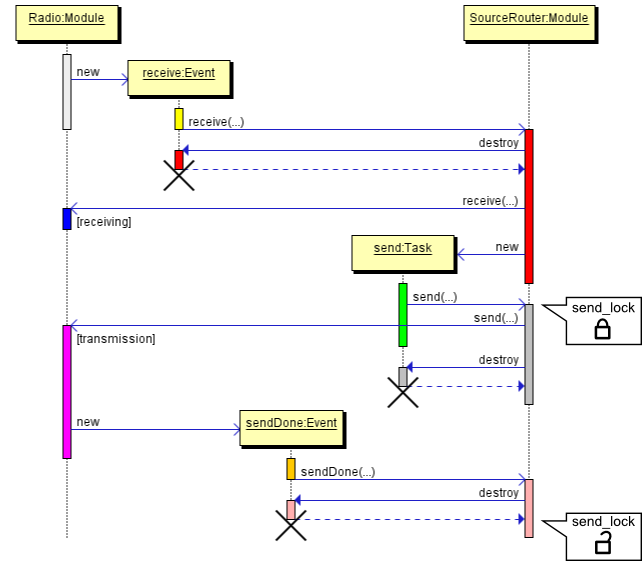
\includegraphics[width=0.8\textwidth]{concurrency.png} 
  \caption{Sequence Diagram of the Mote} 
\label{fig:cncr} 
\end{figure} 
 
\subsection{Network Protocol} \label{ntwprtc}
At its minimum, the simulation must provide source routing mechanism. This means being able to determine the path that the message travels from the source to the destination before issuing the message. The simplest scenario includes one unique omniscient source external to the network which issues message in order to query information from specific mote within the network . Here omniscient refers to the fact that the issuer knows the entire topology of the network so it can encrypt the path in the message prior to its departure. The issuer can also choose different paths to query from the same destination mote.  \\

In this scheme, at each step, an intermediate mote on the path inspects the message to determine the next mote that the message must be sent to. However, since we are working with wireless, devices there is no direct, one-to-one communication between the motes. The packet must be broadcasted at each step and will possibly arrive at multiple surrounding motes. Therefore, motes must have a way of determining whether they are the intended (intermediate or terminal) destination of the packet or not. This is made possible through the suggested message format and communication scheme. 
\subsubsection{Message Format} 
The message in this design has the following construct: 
 
\begin{lstlisting}[label=some-code,caption=Message Construct] 
typedef nx_struct source_route_msg{ 
        nx_uint16_t destid; 
        nx_uint8_t data[256] 
} source_route_msg_t; 
\end{lstlisting} 
 
{\it destid} indicates the intended destination of the packet, in other words "next hob". After each broadcast, receiving motes check this field to determine whether they are the intended destination or not. {\it Data} is a char array of the size 256 which contains the body of the message. However, the first portion of this array contains the remaining path that the message must travel to arrive at its final destination. Assume that the message arrives at a mote with id \begin{math}m_i\end{math} along the path and the final mote's id is \begin{math}m_f\end{math}. This would be the entire content of the maessage: 
 
\begin{figure}[h] 
  \centering 
      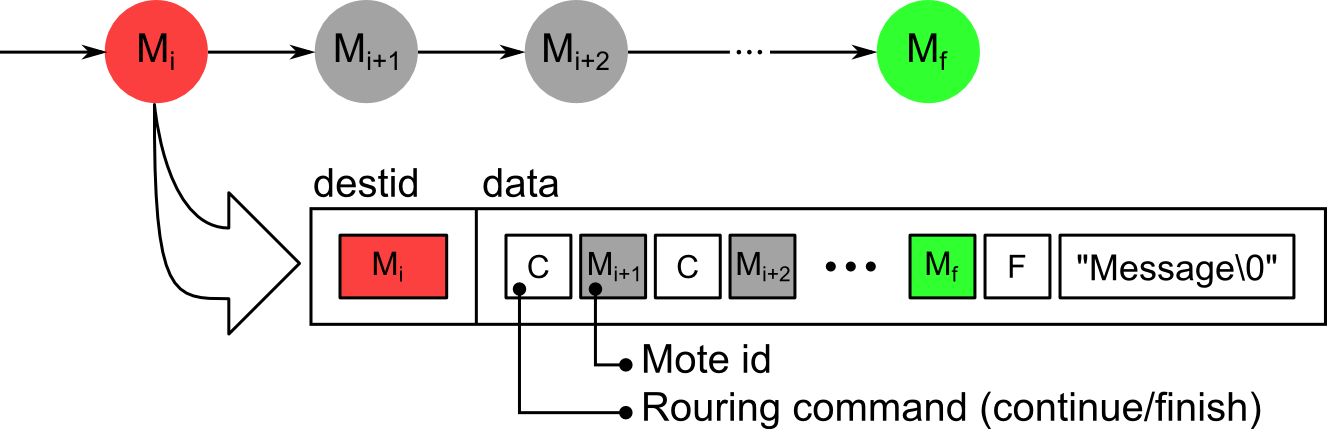
\includegraphics[width=0.8\textwidth]{message_format.png} 
  \caption{Message Format} 
\label{fig:msgfrmt} 
\end{figure} 
 
As it is illustrated in Figure~\ref{fig:msgfrmt}, the first portion of the data array contains a list of command/destination pairs. Next we will explain how the network motes use this message format to route the message through the network. 
 
\subsubsection{Communication Scheme} 
 
After \begin{math}m_i\end{math} in Figure~\ref{fig:msgfrmt} receives the message and confirms that it is in fact the intended destination, it consults the data section of the message to figure out whether the message should be routed further or not. If the first character in the data array is 'F', mote realizes that it is in fact the final destination and the routing process terminates. Alternatively, the character 'C' at the beginning of the array instructs the mote to continue the routing process. In this case, the mote proceeds by converting the second character in the array into a short integer and copying it into a new message's {\it destid} field. This second character in the array  represents the next mote that the message must be sent to. Then, the mote copies the rest of the array (everything after the second index) into the new message's {\it data} field. Finally, the mote braodcasts this new message.\\ 
 

 
Once the message is broadcasted, it might arrive at several surrounding motes. However, each of these motes haveits own unique id. After each of these motes inspect the {\it destid} field of the message, only one of them will accept the message and the rest will drop the message.\\ 
In this design, there is only one active broadcaster at any given time. This active broadcaster is one of the intermediate motes along the route of the message. This communication scheme prevents message duplication. To elaborate on this point further consider the following scenario. Assume \begin{math}m_{i-1}\end{math}, \begin{math}m_{i}\end{math} and \begin{math}m_{i+1}\end{math}  are three consecutive motes on a route that a message takes from its source to its destination. \begin{math}m_{i-1}\end{math}, \begin{math}m_{i}\end{math} and \begin{math}m_{i+1}\end{math} are initially listening for message arrival. Once the message arrives at \begin{math}m_{i-1}\end{math}, it inspects the content of the packet to find out whether it is the intended destination of the message at this point or not. After realizing that is it in fact the intented receiver, it broadcasts the new message intended for \begin{math}m_{i}\end{math} and starts listening once done broadcasting. At this point, all surrounding motes will receive the message but only \begin{math}m_{i}\end{math} accepts it since it is the intended destination of the message. Similarly, as the active broadcaster, \begin{math}m_{i}\end{math} broadcasts the message targeted for \begin{math}m_{i+1}\end{math} while all other motes are listening. The message arrives at \begin{math}m_{i+1}\end{math} and consequently \begin{math}m_{i+1}\end{math} becomes the active broadcaster while all other motes are listening so on and so forth. Figure~\ref{fig:comchm} can help the reader better understand the concept.
\begin{figure}[h] 
  \centering 
      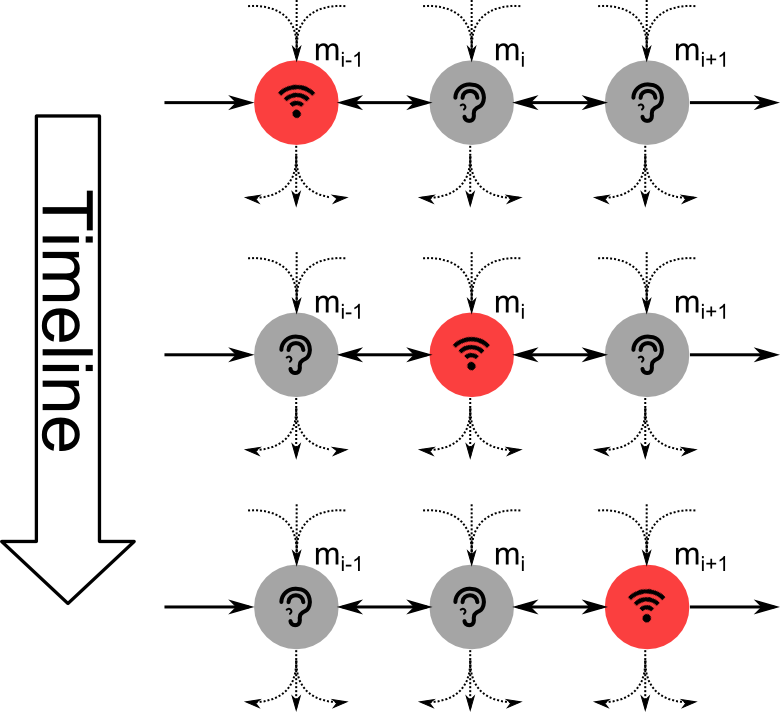
\includegraphics[width=0.5\textwidth]{com_scheme.png} 
  \caption{Singular Broadcaster} 
\label{fig:comchm} 
\end{figure} 
 
This property holds as long the server (original source) issues one message at a time which is true in our scenarios. 
 
 
 
\subsection{Simulation driver} \label{smldrv}
The next step after completing mote's implementation is populating a large number of motes and assemble them together to create the network. To do this, TOSSIM is used. TOSSIM is capable of defining motes, connecting motes to one another, adding noise to the network and injecting messages into the network. However, a driver is needed to instruct TOSSIM to create the specific networks that we desire to use. This driver is written in python. It simply initializes the TOSSIM instance and instruct it to configure the topology of the network based on a provided {\tt *.tpl} file. {\tt *.tpl} files are topology descriptions. They can specify the motes and the connections between them. here is simple {\tt *.tpl} file: 
 
 
\begin{lstlisting}[label=some-code,caption=Sample .tpl File] 
mote 1 
mote 2 
mote 3 
gain 1 2 -30 
gain 2 1 -30 
gain 3 2 -60 
\end{lstlisting} 
 
This topology description maps to the network illustrated in the Figure~\ref{fig:smptpl}. 
 
\begin{figure}[h] 
  \centering 
      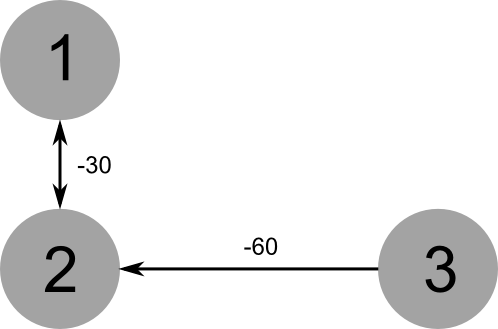
\includegraphics[width=0.3\textwidth]{simple_topo.png} 
  \caption{Simple Topology} 
\label{fig:smptpl} 
\end{figure} 
 
The first portion of the {\tt *.tpl} file describes the motes in the network and their ids. '{\tt mote 1}' means define a new note with id 1. The second portion describes the connections between the motes . '{\tt gain 1 2 -30}' means that when mote 1 transmits data, mote 2 hears it at -30 dBm. Once the topo file is parsed, the network is ready for message injection. This driver can act as the omniscient external source and issue queries to the network. 
 
\subsection{Topologies} \label{tpls}
As mentioned in section~\ref{smldrv}, in order to run the simulation, we must feed it with a {\tt *.tpl} file. The format required by {\tt *.tpl} files is very scriptive and is very prone to make mistakes. More so, some scenarios might require hundreds of motes connected in an arbitrary fashion. This makes it extremely difficult to edit the {\tt *.tpl} file manually. The simulation driver is agnostic of the actual physical structure of the network. It would parse any {\tt *.tpl} file regardless of its semantics as long as it is syntactically correct. This can lead to many network anomalies (ie, topologies that cannot exist in reallity) which further separates the physical and the virtual domains. In order to avoid such situations, a tool is needed to enable the use to model topologies in a realistic manner. This tool must be intuitive and easy to use. 
 
\subsubsection{Requirements} 
The tool must have the following requirement: 
 
 
\begin{itemize} 
\item The user must be able to create topologies of arbitrary size 
\item The user must be able to determin the location of the motes with respect to one another
\item The user must be able to determin the range of each motes signals 
\item The user must be able to connect or disconnect the motes  
\end{itemize} 
The requirements are very visual concepts. Thus a GUI tool is the most intuitive tool and would best fulfill our requirements. We created a Topology Generator tool based on these requirements.
 
\subsubsection{UI Specification} 
 
Figure~\ref{fig:tlpgen} illustrates the Topology Generator's GUI.
 
\newpage 
 
\begin{figure}[h] 
  \centering 
      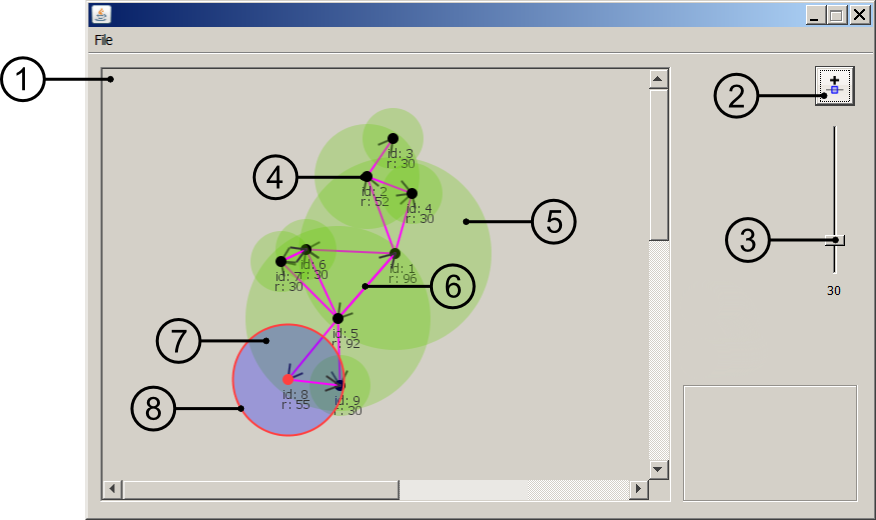
\includegraphics[width=0.8\textwidth]{uiapp.png} 
  \caption{Topology Generator Tool} 
\label{fig:tlpgen} 
\end{figure} 
 
 Here is a brief description of the UI:
\begin{enumerate} 
\item {\bf Map Panel}:\\ This panel is the map of the topology. It represent a physical region in which motes can be positioned. It is an interactive panel which allows the user to manipulate the motes inside it. 
\item {\bf Add mote button}:\\ 
This button allows the user to add new nodes to the map. Once the button is pressed, the user can add a new mote to the map by clicking on the Map panel. The new mote will appear where the user clicked on the map  .
 
\item {\bf Default range slider}:\\This slider determines the default initial range of the the motes when they are being added to the map.
 
\item {\bf Mote center}:\\ This black dot indicates the location of the mote on the map. More so, the user can select the mote by clicking on this dot. 
 
\item {\bf Signal range}:\\ This circle indicates the signal range of the mote.
 
\item {\bf Connection edge}:\\ This edge indicates a connection between two motes. Note that this edge is directed. If mote {\bf A} lies within motes {\bf B}'s range, this edge would be an arrow from {\bf B} to {\bf A}. If they both lie within each other's range this edge would be bi-directional. 
 
\item {\bf Selected mote}:\\ The selected mote appears red with a blue range circle. There is only one selected mote at any given time. User can move the selected mote by dragging its center around the map 
 
\item {\bf Range circumference}:\\ Circumference of the selected mote appears red whenever the pointer gets close to it. The user can drag this circumference toward and away from the mote center to change the range of the selected mote. 
 
\end{enumerate} 

Note that mote connections are automatic in order to maintain the realistic structure of the topology. There is a connection from mote {\bf A} to mote {\bf B} if and only if {\bf B} lies within the range of {\bf A}. The user can enforce a connection by moving one mote into another's range or by expanding the range of one of them so that it would capture the other. In both cases the tool automatically detects and creates the connection. Once the user is satisfied with topology, she can export it as a {\tt *.tpl} file.

\section{Conclusion} 
Here, we simply review what has been accomplished and discuss whether our implementation meets the requirements.
\subsection{Requirement revisited} 
 To refresh our memory, here are proposed requirements:

\begin{enumerate} 
\item Motes are capable of receiving packets 
\item Motes are capable of broadcasting packets 
\item Packets can be routed throughout the network 
\item Motes can be arranged in an arbitrary manner to create various network topologies
\end{enumerate}

In section~\ref{arch}, we explained the architecture of individual motes and in section~\ref{cncrmdl}, we discussed the execution model that the mote adhers to. This mote architecture combined by our concurrent execution model provide the basic send and receive functionalities. Then, we moved on and explained how our proposed message format and communication scheme will facilitate source routing. finally in section \ref{tpls}, by introducing the Topology Generator tool, we enabled the user to create aribtrary topologies on which different scenarios can be run.
 
\subsection{Characteristics and Limitations}  

Before we finish, it is noteworthy to mention certain characteristics and limitations of the simulated networks.
\subsubsection{characteristics}
\begin{itemize}
\item Reliability: the network is not reliable in the general sense since the receiving motes never acknowledge the successfull message receival. There are several situations where a message can be lost. For example, The intended receiver might still be busy processing a message broadcasted from two stages before on the path. Since the radio is busy, the correct message is dropped and will never be revived. Also the noise introduced by TOSSIM might also corrupt the message.
\item Scalability: the network is easily scalable since the routing mechanism of the network is fairly simple. There is only one omniscient source that issues the initial messages. The rest of the motes are agnostic of the structure and the topology of the network. All the information required to route a message is encrypted into the message by the external source. The burden of "valid" routing is on the external source and not the internal motes. So new motes can be added to the network without impacting the logic of routing.
\end{itemize}
\subsubsection{limitation}

\begin{itemize}
\item Bounded path length: The {\it data} field of the message is an array of length 256. Therefore, since each mote to mote transmision requires 2 entries of this array, the maximum path length that a message can travel is 128. 
\item Bounded number of motes: Since each mote id must be representable by a char in the {\it data} field of the message, up tp 128 motes can be addressed.
\end{itemize}

Both of these limitations can be improved by increasing the size of {\it data} field of the message.
  
\bibliographystyle{abbrv}  
 
  
\bibliography{simple}  
\newpage 
 
\begin{thebibliography}{9} 
\bibitem{wsn1}  
John A. Stankovic: Wireless Sensor Networks, {\it University of Virginia}, June 2006

\bibitem{mainppr}  

B. Carbunar, Y. Yu, L. Shi, M. Pearce, V Vasudevan: Query privacy in wireless sensor networks, {\it Applications Research Center, Motorola Labs}

\bibitem{tinyos} 
P. Levis: TinyOS Programming , October 2006

\bibitem{tossim} 
Levis, Phil. "Simulating TinyOS Networks." {\it Computer Science Division}. Web. 26 Apr. 2012. [http://www.cs.berkeley.edu/~pal/research/tossim.html]
 
\end{thebibliography} 
  
\end{document}